\chapter{Introduction}\label{chapter:introduction}
The oxford English dictionary defines provenance as the place of origin or earliest known history of something. An example of provenance can be seen with a college transcript. A transcript can be defined as the provenance of a college degree because it outlines all of the courses satisfied in order to attain the degree.

\par In the field of computing, data provenance also known as data lineage can be defined as the history of all transformations performed on a data object from the its creation to its current state. Data Provenance has been explored in the areas of scientific computing to track how an experiment is reproduced, in buisness to determine the workflow of  processes, in field of computer security for forensic analysis and intrusion detection. Provenance denotes the who, where and why of data.An example of provenance for software systems is a web server's log file. This file contains metadata for various request and response time and ip addresses of all host systems that tries to request information from the server.Provenance data is represented as an acyclic graph which denotes casual relationship and dependencies between entities.Provenance ensures trust and integrity of data. The information in which provenance offers can be used in digital forensics to investigate the cause of a malicious attack and also in intrusion detection systems to further enhance the security of computing devices.  \textcolor{blue}{Most IoT devices are memory constrained devices} \textcolor{red}{TODO: Expand more on statement.}.

 
\textcolor{red}{TODO: Create transition from Data provenance to IoT...}


The internet of things(IoT) can be defined as a network of heterogeneous devices communicating together. With the recent data explosion,information is ubiquitous and  disseminated at vast rate. Making IoT systems provenance aware is of the essence because it ensures trust and  integrity of systems. Enabling IoT device provenance aware allows devices to be able to capture information such as the who, where and how transformations occur on a data object which enables  backtracking in an event of a malicious attack.



\section{Motivation}
According to a report released by Cisco, it is estimated that a total of 50 million devices will be
connected to the internet by the year 2020. With the vast amounts of heterogeneous devices connected,
security and privacy risks are inceased. Rapid7, an  IT security and analytics organization, released a report. In their report, they outline that vulnerabilities exist in
baby monitors which allowed intruders unauthorized remote access to these devices
whereby an malicious intruder can remotely view live video feeds from the device. Having a provenance aware
system will be beneficial in this situation since we have a record of input and output
operations performed on the device, we can be able to look back on operations
performed on the device to determine who, where, and how a malicious activity
occurred. Most of the devices (things) connected in an IoT network are embedded systems, which
require lightweight and efficient solutions compared with general purpose
systems.
This requirement is attributed to the constrained memory and computing of such
devices. A major issue arises in ensuring that data is properly secured and
disseminated across the IoT network. The vast amount of data generated from IoT
devices requires stronger levels of trust which can be achieved through data
provenance. Provenance has immense benefits in IoT. Data provenance ensures
authenticity, integrity and transparency between information disseminated across an
IoT network. Security applications such as intrusion detection, digital forensics, and
access control can be further enhanced by incorporating data provenance in IoT. The goal of data provenance is to determine causality and effect of actions or
operations performed on a data object. Provenance ensures transparency between things
connected in IoT systems. By creating data transparency, we can trace information to
determine where, if and when a malicious attack occurs. To achieve transparency, we
propose a secure provenance aware system that provides a detailed record of all data
transactions performed on devices connected in an IoT network and also investigate its applications in providing intrusion detection to IoT devices.  \textcolor{red}{Data is generated in at a fast rate in real-time by sensors and actuators. The provenance of this data tends to be larger than the data itself.}

Metada

\subsection{Provenance and Metadata}
Metadata and provenance are often related but yet have subtle differences. Metadata contains descriptive information about data objects. Metadata can be considered as provenance when there exists relationship between objects and explains how objects are . For example a web server can have metadata information such as the host and destination IP addresses which might not be considered as provenance information for a specific application.It could also contain time stamps with loction of IP addresses which are considered as provenance information. In summary metadata and provennace are not the same, metadata contains valuable  provenance information but not all provenance information is metadata. 


\textcolor{red}{Metadata is used to represent properties of objects. Many of those properties have to do with provenance, so the two are often equated. How does metadata relate to provenance?
Descriptive metadata only becomes part of provenance when one also specifies its relationship to deriving an object. For example, a file can have a metadata property that states its size, which is not considered provenance information since it does not relate to how it was created. The same file can have metadata regarding creation date, which would be considered provenance-relevant metadata. So even though a lot of metadata has to do with provenance, both terms are not equivalent. In summary, provenance is often represented as metadata, but not all metadata is necessarily provenance.}


\subsection{Provenance and Log data}
Log data contains information about that activity of an object in a operating system or process.Provenance is a specialized form of Log data. It contains information specific to an application domain. Log files might contain unrealted information such as error messages, warnings which might not be considered as provenance data. Logging is limited, lacking information that shows the internal state of an object. Provenance allows for a holistic collection of information that relates to the change the internal state of an object.

\section{Provenance-Aware IoT Device Use Case}

Consider a smart home which contains interconnected devices such as a thermostat connected a wireless network. This device automatically detects and regulates the temperature of a room based on prior information of a user's temperature settings, a smart lock system that can be controlled remotely and informs a user via text when has been a breach, a home security camera motoring system, A smart fridge which sends a reminder when food produce are low. A malicous intruder tries to gain access to the smart lock system and security camea remotely. Provenance can be used to track the series  of events to determine where and how a malicious attack originated.It can also be used as a safeguard to alert of a possible remote or insider compromise thereby protecting us from future or current malicious attacks.

\begin{figure}[h!]
\begin{center}

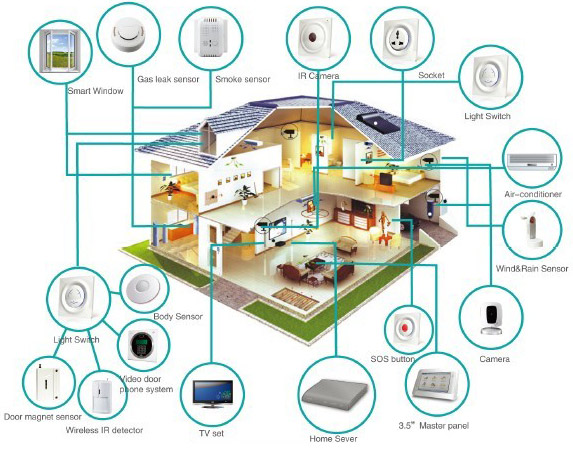
\includegraphics[height=3in]{smarthome-diagram.png}
\end{center}
\caption{Place holder for use case Diagram}

\end{figure}






\section{Research Questions}
collecting provenance data in IoT devices raises some key research issues. Some of these issues raised are outlined below:

\begin{itemize}

\item Memory constraints on IoT Devices: The vast amounts of data generated leads high storage space utilization . Proper memory management/data pruning techniques should be employed for efficient storage of data on memory contrained devices. 

\item How do we model provenance data for IoT devices? Do we use the OPM approach or create a specialized taxonomy for modeling provenance data.

\item Provenance Query: How do we query provenance data in order to interprete provenance information and make anaylsis of data collected.

\item Provenance Versioning: Provenance version creates cycles. When a file is read or edited do we create a new instance of the file? Tracking all transformations that occurs on a data object in memeory constrained devices might lead to running out of storage space. A new instance of the provenance of that file should be created and included in the provenance data.

\item Securing Provenance: Due to the great level of sensitivity that  provenance data entails, it is of utmost importance to ensure the confidentiality and integrity of provenance data stored on IoT devices while at rest or in transit. Proper encryption and authentication techniques need to be employed to ensure the confidentiality, integirty, and availability of provenance data.

\item Provenance collection raises privacy issues.How do we ensure that the vast amount of data collected is not invasive to the privacy of the use and also is not used as a tool to perform malicious attacks.
\end{itemize}

\section{Research Contribution}

In this dissertation, we proposes the following key contributions:

\begin{itemize}
  \item A provenance collection framework which denotes causality and dependencies between entities contained in an IoT system.This system creates the groundwork for capturing and storing provenance data  on IoT devices.
  \item A novel framework for data storage on embedded systems.This addresses the storage issues of the memory constrained IoT devices.
   \item A framework for providing intrusion detection using provenance data in an IoT eco system.
\end{itemize}

\section{Organization of Dissertation proposal}

The remaining portion of the dissertation proposal is organized as follows.  Chapter 2 talks about background information on data provenance, some of the techniques involved in collecting system level provenance, data pruning techniques for storage optimization and also applications of data provenance with provenance based intrusion detection system. chapter 3 discusses our proposed provenance collection system and focuses specifically on preliminary work done in creating a provenance aware system. Chapter 4 concludes the proposal and discusses the proposed framework and projected timeline for completion.

